\documentclass{beamer}
\usetheme{default}
\usepackage{tikz}
\usepackage{subfig}
\setlength{\unitlength}{\textwidth} 
\tikzstyle{vertex}=[auto=left,circle,fill=black!25,minimum size=20pt,inner sep=0pt]
\title[Blockmodels for relational events]%(optional, only for long titles)
{Stochastic blockmodels for relational events}
\subtitle{}
\author[DuBois, Christopher] % (optional, for multiple authors)
{Christopher~DuBois\inst{1} \and Carter~Butts\inst{2} \and Padhraic~Smyth\inst{3}}
\institute[] % (optional)
{
  \inst{1}%
Department of Statistics \\
University of California, Irvine
  \and
  \inst{2}%
Department of Sociology \\
University of California, Irvine
  \and
  \inst{2}%
Department of Computer Science \\
University of California, Irvine
}
\date[Sunbelt 2012] % (optional)
{Sunbelt 2012}
\subject{Informatik}
\begin{document}
\frame{\titlepage}

\begin{frame}{Dyadic event data}
\begin{figure}
{
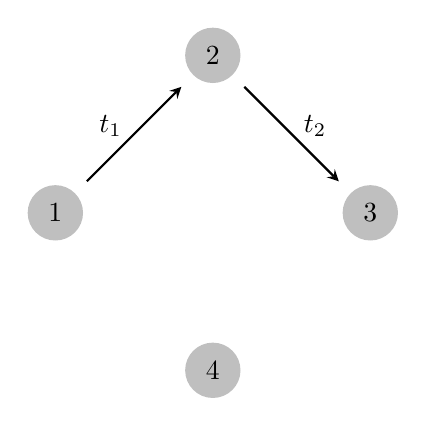
\begin{tikzpicture}[scale=1,transform shape,thick]
  \node[vertex] (n1) at (0,0)  {1};
  \node[vertex] (n2) at (2,2)  {2};
  \node[vertex] (n3) at (4,0) {3};
  \node[vertex] (n4) at (2,-2) {4};
\draw[-stealth] (.4,.4) -- (1.6,1.6);
\draw[-stealth] (2.4,1.6) -- (3.6,.4);
\node at (.7,1.1) {$t_1$};
\node at (3.3,1.1) {$t_2$};
\end{tikzpicture}
}
\end{figure}

\begin{itemize}
\item Above example: 2 dyadic events occurring among 4 nodes
\item Nodes may have covariates
\item Interested in inferences about the rate of particular events, conditioned on what we have observed
\end{itemize}
\end{frame}

\begin{frame}{Relational event models}

Multiplicative models for the hazard:
$$\log \lambda_{ij}(t | \cdot) = \boldsymbol{\beta}' \mathbf{s}(t,i,j)$$

Likelihood:

\begin{align}
\mathcal{L}(\mathcal{A}|\theta) &= \prod_{m=1}^M \lambda_{i_m,j_m}(t_m|\cdot) \prod_{(i,j) \in \mathcal{R}}\exp\{ - (t_m - t_{m-1}) \lambda_{ij}(t_m | .) \}
\end{align}

\begin{itemize}
\item $M$: number of events
\item $t_m$: time of event $m$
\item $\mathcal{R}$: set of dyadic events
\end{itemize}

\end{frame}


\begin{frame}{Stochastic blockmodels}

\begin{itemize}
\item Each actor belongs to a latent class. 
\item Model block-wise interactions (mixing rates).
\end{itemize}

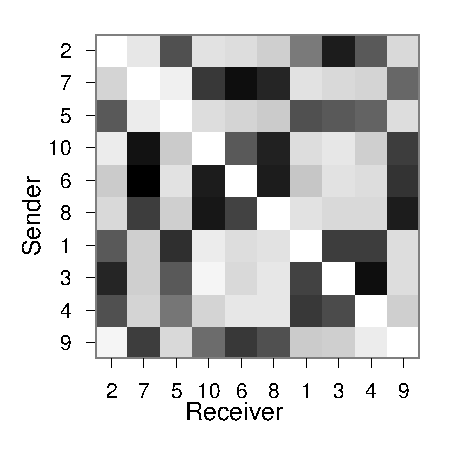
\includegraphics[scale=.45]{../../figs/synthetic/unsorted}
\uncover<2->{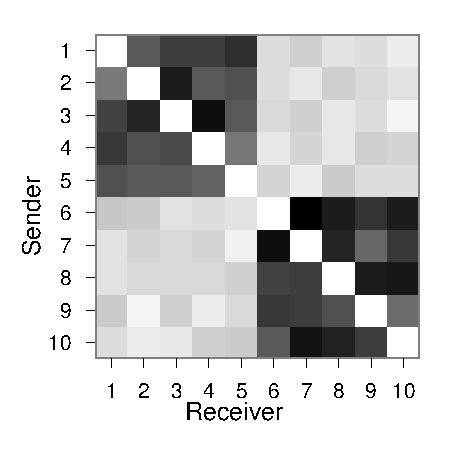
\includegraphics[scale=.45]{../../figs/synthetic/mat}}
\uncover<3->{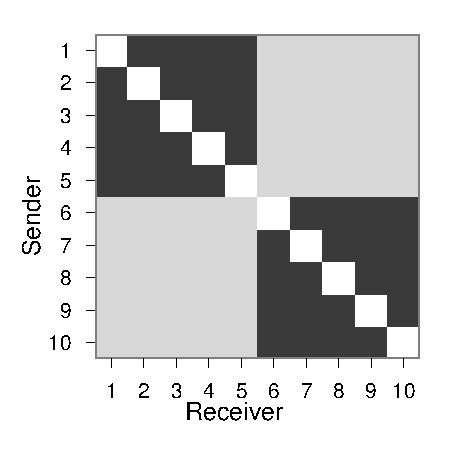
\includegraphics[scale=.45]{../../figs/synthetic/bm} }

\vspace{-.8cm}
\begin{align*}
\uncover<4->{
\mbox{Mixing rates} & & \boldsymbol{\eta} =& \left[
\begin {array}{cc}
 \eta_{11}& \eta_{12} \\
 \eta_{21}& \eta_{22} 
\end {array}
\right]
= \left[
\begin {array}{cc}
.8 & .2\\.2 & .8
\end {array}
\right] \\
}
\uncover<5->{
\mbox{Dyad (i,j)} &  & y_{ij} \sim& F(\eta_{z_i,z_j}) \\
}
\uncover<6->{
\mbox{Actor i's class} & & z_i \sim& \mbox{Categorical}(\pi)
}
\end{align*}

\end{frame}


\begin{frame}{Stochastic blockmodels for relational event data}
Idea:
  \begin{itemize}
  \item Assume each actor $i$ belongs to a latent class $z_i$.
  \item Model event dynamics between blocks.
  \end{itemize}

\begin{align}
\log \lambda_{ij}(t | \mathcal{A}_t,\mathbf{z}) = \boldsymbol{\beta}_{z_i,z_j} \mathbf{s}(t,i,j|\mathcal{A}_t,\mathbf{z}).
\end{align}

\uncover<2>{Notation:
\begin{itemize}
\item $\boldsymbol{\beta}_{k,l}$: parameter vector for relational events from an actor in block $k$ to an actor in block $l$
\item  $\mathcal{A}_t$: history prior to time $t$
\item $\mathbf{z}$: vector of class assignments
\end{itemize}
}

\uncover<3>{
\vspace{-3cm}
Benefits:  
\begin{itemize}
\item Adjust for unobserved heterogeneity.
\item Obtain clusters of nodes who have similar interaction dynamic with other parts of the network.
\end{itemize}

}

\end{frame}

\begin{frame}{Model specification for $X_{ij}(t)$}
\textbf{Participation shifts} adjust for the next event
\begin{itemize}
\item AB-BA
\item AB-BY
\item AB-AY
\item AB-XA
\item AB-XB
\end{itemize}

\textbf{Degree effects} count the number of previous events
\begin{itemize}
\item sent by sender
\item received by sender
\item sent be receiver
\item received by receiver
\item previous occurrences
\end{itemize}

\end{frame}

\begin{frame}{Specifying degree effects (and explosion)}

\end{frame}

\begin{frame}{Scalability}
Only use covariates for $(i,j)$ that involve either $i$ or $j$.

\begin{figure}
\centering 
%\subfigure[Dynamic network data]
%{
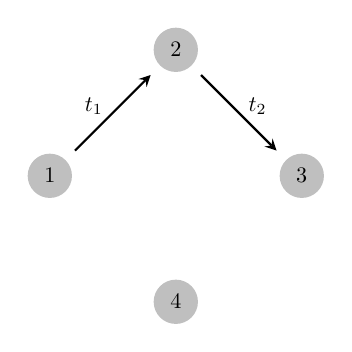
\begin{tikzpicture}[scale=.8,transform shape,thick]
  \node[vertex] (n1) at (0,0)  {1};
  \node[vertex] (n2) at (2,2)  {2};
  \node[vertex] (n3) at (4,0) {3};
  \node[vertex] (n4) at (2,-2) {4};
\draw[-stealth] (.4,.4) -- (1.6,1.6);
\draw[-stealth] (2.4,1.6) -- (3.6,.4);
\node at (.7,1.1) {$t_1$};
\node at (3.3,1.1) {$t_2$};
\end{tikzpicture}
% }
% \subfigure[Intensities for two dyads]
% {
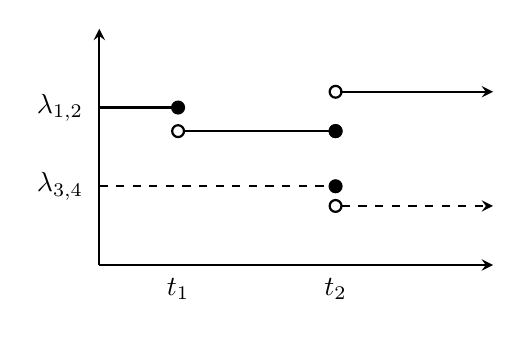
\begin{tikzpicture}[scale=1,transform shape,thick]
\draw[-stealth] (0,0) -- (0,3);
\draw[-stealth] (0,0) -- (5,0);

% First timeline
\draw (0,2) -- (1,2);
\draw[fill=black] (1,2) circle (0.75mm);
\draw (1,1.7) circle (0.75mm);
\draw (1.08,1.7) -- (3,1.7);
\draw[fill=black] (3,1.7) circle (0.75mm);
\draw (3,1.7) circle (0.75mm);
\draw (3,2.2) circle (0.75mm);
\draw[-stealth] (3.05,2.2) -- (5,2.2);

% second timeline
\draw[dashed] (0,1) -- (3,1);
\draw[fill=black] (3,1) circle (0.75mm);
\draw (3,.75) circle (0.75mm);
\draw[dashed, -stealth] (3.08,.75) -- (5,.75);

% labels
\node at (-.5,2) {$\lambda_{1,2}$};
\node at (-.5,1) {$\lambda_{3,4}$};
\node at (1,-.3) {$t_1$};
\node at (3,-.3) {$t_2$};
\end{tikzpicture}
%}
\end{figure}

\begin{itemize}
\item Restricts the class of effects one can use
\item Complexity of likelihood computation reduced ($N^2 \rightarrow N$)
\end{itemize}
\end{frame}

\begin{frame}{Synthetic example: 2000 events among 10 actors}
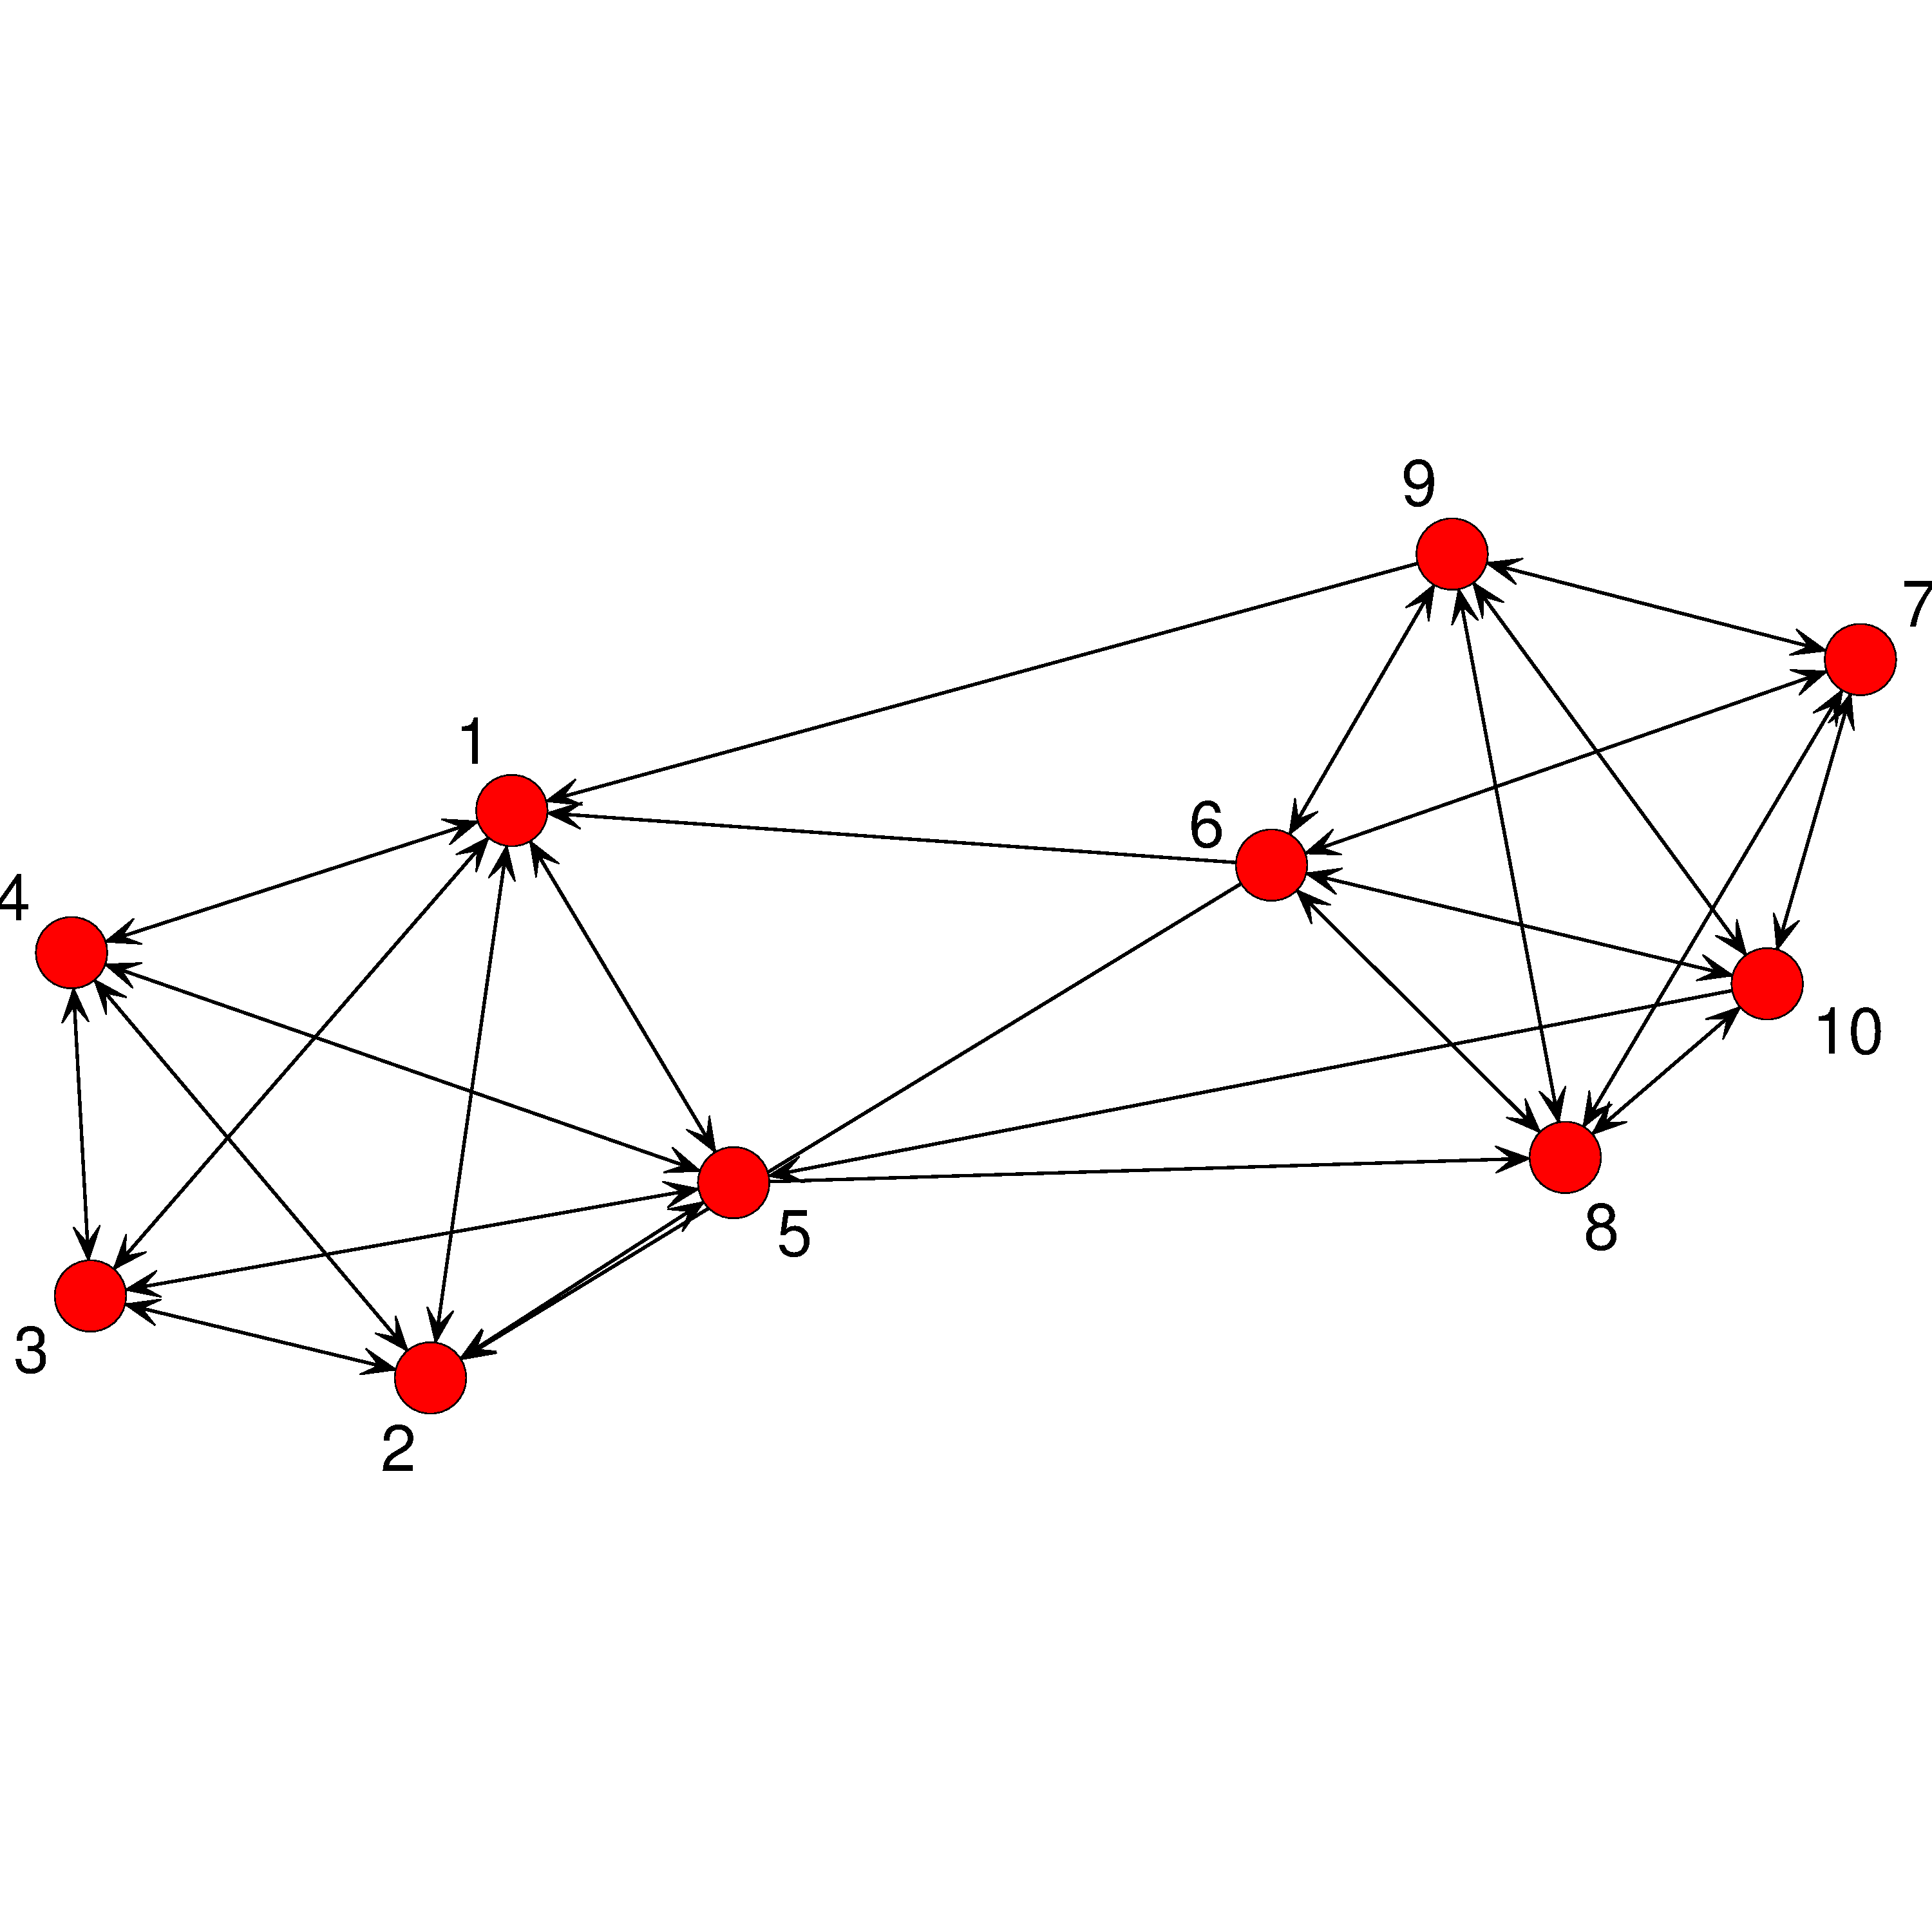
\includegraphics[scale=.12]{../../figs/synthetic/network}
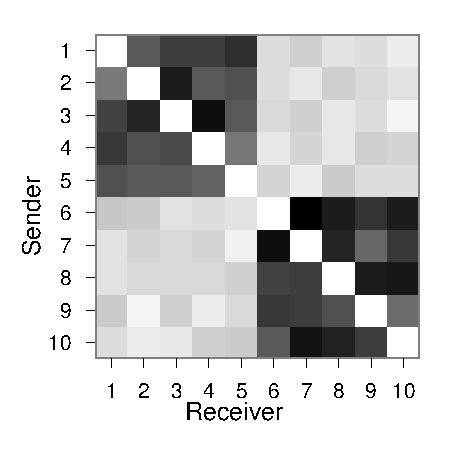
\includegraphics[scale=.7]{../../figs/synthetic/mat}
\end{frame}


\begin{frame}{Synthetic example: $\beta$ and observed counts}
\begin{picture}(0.0,0.0)
   \put(-.1,-0.25){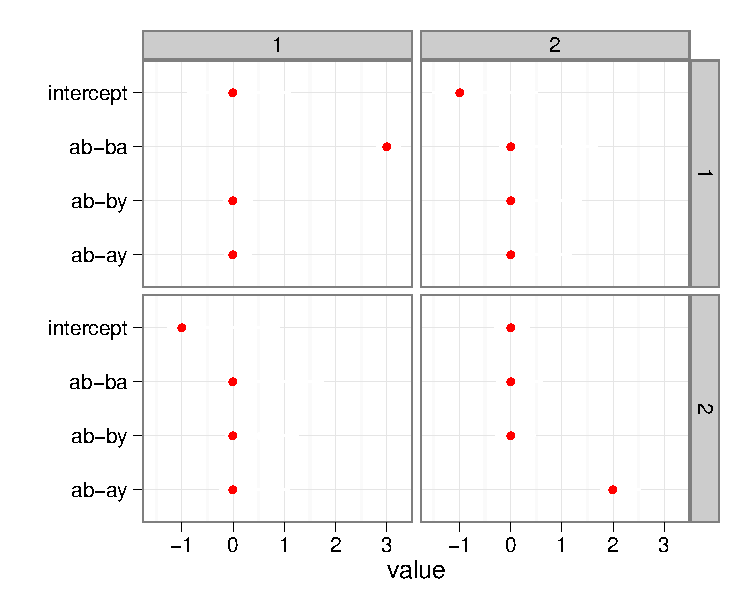
\includegraphics[width=0.7\textwidth]{../../figs/synthetic/params-true}}
   \put(.6,-0.3){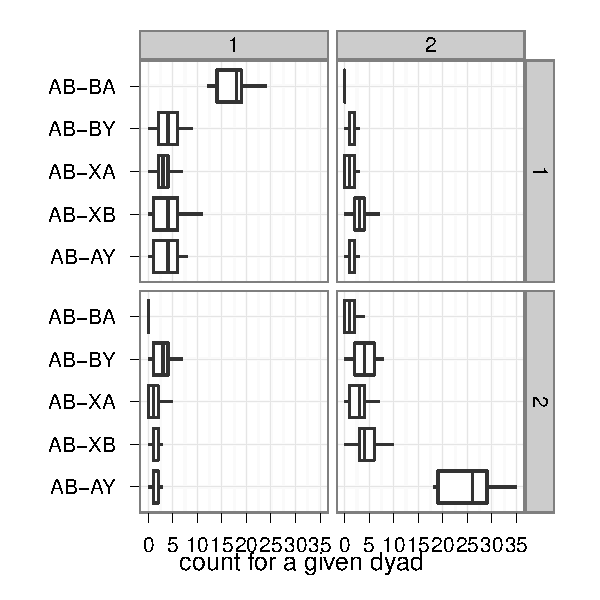
\includegraphics[width=0.5\textwidth]{../../figs/synthetic/counts}}
\end{picture}
\end{frame}


\begin{frame}{Synthetic example: slice sampling for $\hat{\beta}$ and Gibbs on
    $\mathbf{z}$}
\begin{picture}(0.0,0.0)
   \put(-.1,-0.25){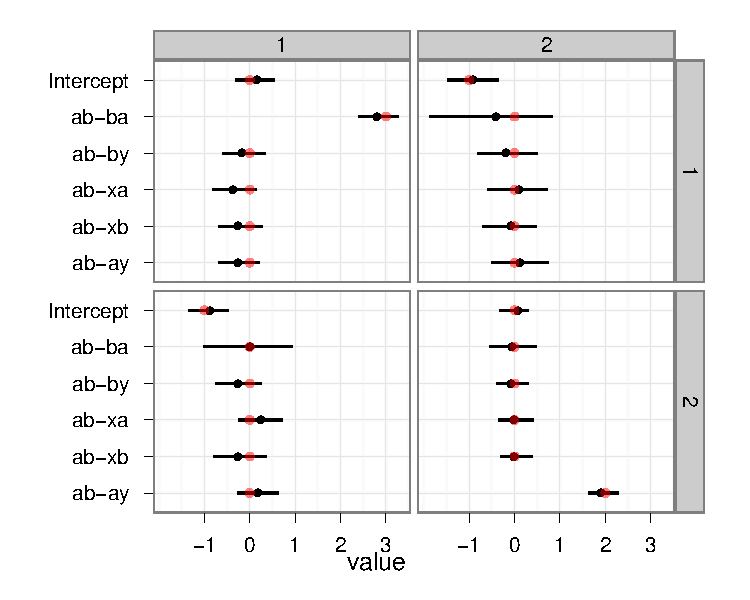
\includegraphics[width=0.7\textwidth]{../../figs/synthetic/params-estimates}}
   \put(.6,-0.3){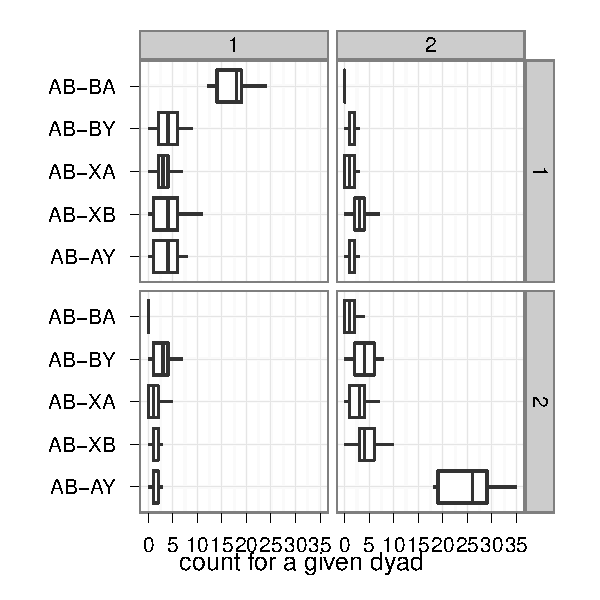
\includegraphics[width=0.5\textwidth]{../../figs/synthetic/counts}}
\end{picture}

%\vspace{1in}
%From 100 samples after 50 burnin using Gibbs sampling for $\mathbf{z}$ and slice sampling for $\boldsymbol{\beta}$).
\end{frame}


\begin{frame}{Application: Dyadic interactions on Twitter}
  \begin{itemize}
  \item Tweets from Twitter.com occurring between from May 11, 2009 to January 26, 2012 with hashtag \texttt{\#rstats}.
  \item Selecting tweets beginning with the \texttt{@} symbol, and mark the first mentioned user as the recipient.
  \item Of 28337 total tweets in this time period, 3926 were directed events among a total of 1079 users.
  \item We consider a subset 487 users who participated in more than one event, using a training set of 2000 events and a test set of 1330 events.
  \end{itemize}
\end{frame}

\begin{frame}{Application: Dyadic interactions on Twitter}
Prediction experiments and model comparison
\end{frame}

\begin{frame}{Application: Dyadic interactions on Twitter}
Plot parameter estimates for winning model
Compare to fitting a single relational event model
\end{frame}

\begin{frame}{Discussion}
Interpretation of parameter estimates
  \begin{itemize}
  \item Method clusters with respect to the relational event dynamics for a set of actors
  \end{itemize}

Main takeaways
\begin{itemize}
\item Detailed, highly dependent model for local structure\\ (using relational event models)
\item Latent variable model to capture meso-level structure \\(using stochastic block model)
\end{itemize}
\end{frame}

\begin{frame}{Future directions}
  \begin{itemize}
  \item Benefits of mixed-membership ideas
  \item Dirichlet process instead of fixed $K$ (with split-merge sampling?)
  \end{itemize}
\end{frame}

\begin{frame}{References}
  
\end{frame}

\end{document}
